%        File: sum11.tex
%     Created: 1/19/2011 
\documentclass{anstrans}
%%%%%%%%%%%%%%%%%%%%%%%%%%%%%%%%%%%
\title{Open Architecture and Modular Paradigm of \Cyclus, a Fuel Cycle Simulation Code}
\author{Kathryn D.~Huff, Paul P.H.~Wilson, Matthew J.~Gidden}

%% uncomment these next five only if using anstrans
\institute{Department of Nuclear Engineering \& Engineering Physics, University of Wisconsin, Madison, WI, 53706}
\email{khuff@cae.wisc.edu}
\usepackage{graphicx}
\usepackage{booktabs} % nice rules for tables
\usepackage{microtype} % if using PDF
\newcommand{\units}[1] {\:\text{#1}}%
\newcommand{\SN}{S$_N$}%{S$_\text{N}$}%{$S_N$}%
\newcommand{\Cyclus}{\textsc{Cyclus }}


\date{}
\begin{document}

%%%%%%%%%%%%%%%%%%%%%%%%%%%%%%%%%%%
\section{Introduction}
The \Cyclus project at the University of Wisconsin - Madison is the result of lessons learned from experience with previous nuclear fuel cycle simulation platforms. The current version is an object oriented C++ application with XML-based pre-processing. Key concepts in the design of \Cyclus include open access to the simulation engine, modularity with regard to functionality, and relevance to both scientific and policy analyses. \textbf{The combination of modular encapsulation within the software architecture and an open development paradigm allows for collaboration at multiple levels of simulation detail and data security.}

%%%%%%%%%%%%%%%%----------%%%%%%%%%%%%%%%%%%%
\section{Software Architecture and Development}

%%%%%%%%%%%%%%%%%%%%%%%%%%%%%%%%%%%%%%%%%%%%%%%%%%%%%%%%%%%%%%%%%%%%%%%%%%%%%%%%
\subsection{Open Development Paradigm}
\Cyclus obeys an open development paradigm that utilizes current best practices in distributed code development and facilitates inter-institutional collaborations. The \Cyclus development framework employs a modern, open source philosophy that ensures transparency, attracts contribution from a varied community of collaborators, and guarantees institution-independent access to all potential users. 

A public source-code repository provides unhindered access to the fundamental simulation framework and basic fuel-process models volunteered by developers. Granting unfettered access only to the \Cyclus engine allows for separation of the source code from any input data, thereby allowing secure and proprietary model developers to be similarly encouraged to utilize the \Cyclus framework. This modern development model passively distributes specialized content to interested research groups, and facilitates parallel model development efforts by institutions with complimentary goals. The transparency inherent in this type of open source development path also facilitates code review by exposing available content to verification and validation by collaborators with diverse areas of specialization and levels of expertise.

This process also benefits from the ability to identify and utilize third-party, open-source libraries when such libraries provide necessary additional functionality. Thus far, such libraries have been used to provide basic infrastructure functionality such as file input/output, as well as model-specific capabilities for advanced network flow optimization. An indepently developed integer programming module is an example of one such addition.

\begin{figure}[h]
  \begin{center}
    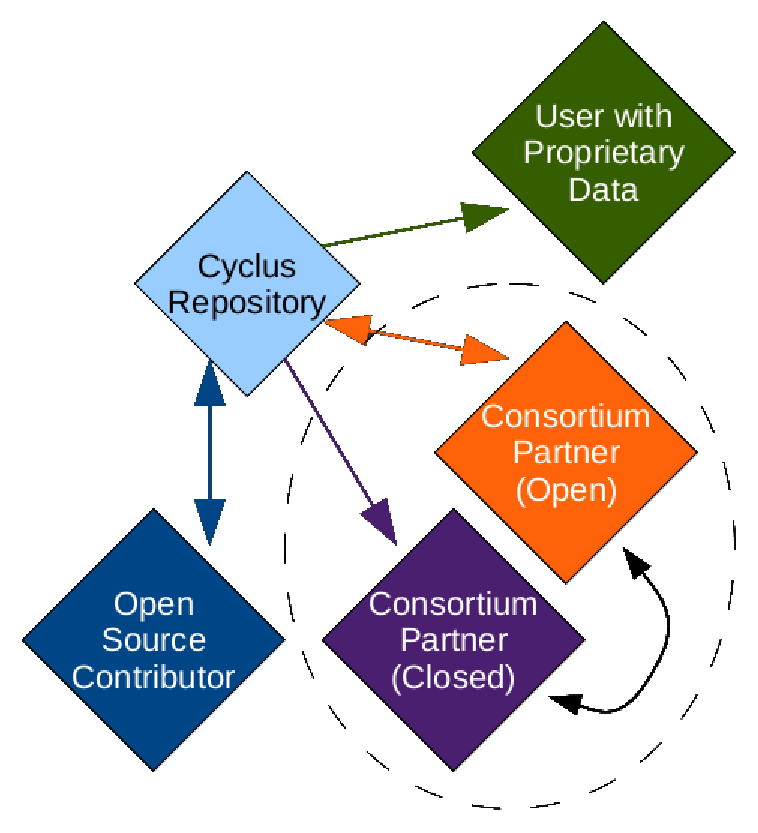
\includegraphics[height=7cm]{openness.eps}
  \end{center}
  \caption{\Cyclus Open Repository Paradigm}
  \label{fig:openness}
\end{figure}
%%%%%%%%%%%%%%%%%%%%%%%%%%%%%%%%%%%%%%%%%%%%%%%%%%%%%%%%%%%%%%%%%%%%%%%%%%%%%%%%
\subsection{Dynamic Module Loading}
The ability to dynamically load independently constructed modules is a heavy focus of \Cyclus development. Dynamically-loadable modules are the primary mechanism for extending \Cyclus' capability. The primary benefit of this approach is encapsulation: the trunk of the code is completely independent of the individual models. Additionally, any customization or extension is implemented only in the loadable module. A secondary benefit of this encapsulation is the ability for contributors to choose different distribution and licensing strategies for their contributions. By allowing models to have varied availability, the security concerns of developers can be assuaged. Finally, this strategy allows individual developers to explore different levels of complexity within their modules, including wrapping other simulation tools as loadable modules for \Cyclus. This last benefit of dynamically-loadable modules addresses another goal of \Cyclus: ubiquity amongst its potential user base. By engineering \Cyclus to easily handle varying levels of complexity, a single simulation engine can be used by both users keen on big-picture policy questions as well as users interested in more detailed, technical analyses.

%%%%%%%%%%%%%%%%%%%%%%%%%%%%%%%%%%%%%%%%%%%%%%%%%%%%%%%%%%%%%%%%%%%%%%%%%%%%%%%%
%%%%%%%%%%%%%%%%----------%%%%%%%%%%%%%%%%%%%
\section{Modeling Paradigm}
The modeling paradigm adopted by \Cyclus includes a number of fundamental concepts which comprise the bedrock on which other, more flexible, design choices have been made. %The majority of these relatively inflexible, basic concepts encompass the differientation of fuel-cycle models in the literature. Each concept was chosen after a careful review of the available literature and the filtering of said literature by the above stated goals of the \Cyclus project.  %% I don't understand what you're trying to say here. The inflexible things are the structural requirements for a universal modular interface. We consulted no literature. Anthony broke GENIUS when he tried to add bright and we decided we needed a more modular code. For modularity (and encapsulation), you need a concretely defined module interface. Perhaps the following is more truthy.. 


%%%%%%%%%%%%%%%%%%%%%%%%%%%%%%%%%%%%%%%%%%%%%%%%%%%%%%%%%%%%%%%%%%%%%%%%%%%%%%%%
\subsection{Discrete Materials and Facilities}
The \Cyclus modeling infrastructure is designed such that every facility in a global nuclear fuel cycle is treated and acts individually. While modeling options will exist to allow collective action, this will be as a special case of the individual facility basis. Each facility has two fundamental tasks: the transaction of goods or products with other facilities and the transformation of those goods or products from an input form to an output form. 
%%%%%%% Perhaps these examples can be more brief. . . %%%%%% 
%%%%%%% For instance, a fuel fabrication facility may receieve enriched Uranium Hexaflouride (UF$_{6}$) from an enrichment facility and provide fuel assemblies to a reactor facility. These materials will be modeled as discrete objects that exist for a finite time and whose composition and transaction history is logged throughout the simulation. In the previous example, the discrete objects include barrels of enriched UF$_{6}$ and entire fuel assemblies.

%%%%%%%%%%%%%%%%%%%%%%%%%%%%%%%%%%%%%%%%%%%%%%%%%%%%%%%%%%%%%%%%%%%%%%%%%%%%%%%%
\subsection{Market-based Material Transactions}
The transaction of nuclear materials takes place in markets that act as brokers matching a set of requests for material with a set of offers for that material. A variety of market models will be available to perform this brokerage role. It is important to note that each market is defined for a single commodity and acts independently of other markets. Once the requests and offers have been matched by each market in a simulation, the facilities exchange material objects.

%%%%%%%%%%%%%%%%%%%%%%%%%%%%%%%%%%%%%%%%%%%%%%%%%%%%%%%%%%%%%%%%%%%%%%%%%%%%%%%%
\subsection{Region-Institution-Facility Hierarchy}
Many times in a fuel-cycle simulation, parameters describing relationships between facilities are required. For instance, one may wish to account for the presence of a contract between two facilities, or one may wish to model two facilities operated by the same entity. Accordingly, \Cyclus implements this ability via a Region-Instituion-Facility hierarchy. Every discrete facility in \Cyclus is considered to be owned by an institution that operates in a geographic region.  An institution can be used to represent any entity that may own and operate a facility such as a private corporation, a government agency, or a non-governmental organization, among others.  A region can be used to represent any geographic area, typically a politically relevant area such a sub-national region (e.g. a U.S. State), a nation state (e.g. South Korea), or a supranational region (e.g. the E.U.).  While some performance parameters of the facility may depend on its institutional ownership or geographical location, this capability is more useful in modeling the way in which a facility engages in a market for trade of nuclear material based on its ownership entity and/or region.

%%%%%%%%%%%%%%%%%%%%%%%%%%%%%%%%%%%%%%%%%%%%%%%%%%%%%%%%%%%%%%%%%%%%%%%%%%%%%%%%
\subsection{Optimization and Sensitivity}
System optimization is the general goal of a simulation modeling tool. It is important, however, to recognize the differences between macroscopic and microscopic intstances of optimization that exist in such a fuel-cycle simulation. If one treats individual entities as decision makers who choose to optimize some local objective function, it is entirely possible and likely that such a model will provide a different end state than a simulation optimizing a system globally. In general, the former scenario is quite complicated and may include both game theoretical models as well as input from more qualitative fields. The latter instance can be applied in a more scientifically rigorous manner, but may not (and in fact most likely will not) account for the needs or wants of an individual actor in the simulation.

Accordingly, \Cyclus is currently being developed under the following assumption: a user is interested in a single simulation with a large, multi-dimensional data set which allows modern optimization technology to seek globally optimal solutions based on global objective functions. Since institutional decision making tends to seek an optimal solution only for the actor making that decision (local or microscopic optimization), it may not lead to an outcome that optimizes for the largest population of stakeholders. There are plans to provide both such capabilities to \Cyclus, as a user interested in more politically-relevant inquiries may be more interested in a agent-based decision making model; however, in order to develop and benchmark initial functionality, global optimization is being given priority.

%%%%%%%%%%%%%%%%%%%%%%%%%%%%%%%%%%%%%%%%%%%%%%%%%%%%%%%%%%%%%%%%%%%%%%%%%%%%%%%%
%%%%%%%%%%%%%%%%----------%%%%%%%%%%%%%%%%%%%
\section{Conclusions}
The above sections outline a proposed fuel cycle simulation platform currently under development at the University of Wisconsin at Madison. \Cyclus presents an effective framework for transparent, accessible, yet compartmentalized code development. Its software architecture and modeling paradigm promises to maximize ease of use, ease of contribution, technical utility, and relevance to both technical and policy-based inquiries, which may represent an optimal way forward for the next generation of nuclear fuel cycle modeling.
%%%%%%% Faith in the scientific analysis of future nuclear fuel cycles and the political decision making process thereof is easily garnered via such pillars of conceptual design.
%%%%%%% What a sentence! I like it, but I think it's a little florid for this forum. . . 
%%%%%%% As Paul Dirac once said. . . In science one tries to tell people, in such a way as to be understood by everyone, something that no one ever knew before. But in the case of poetry, it's the exact opposite!



%%%%%%%%%%%%%%%%%%%%%%%%%%%%%%%%%%%
\nocite{huff_cyclus:_2010}
\bibliographystyle{ans} 
\bibliography{bibliography}
\end{document}


